\documentclass{beamer}
\usetheme{metropolis}
\usepackage{tikz}

\title{\vspace{4em}Automated Maze Solver}
\subtitle{CSE 316: Microcontroller and Microprocessor Sessional}
\author{
  \textbf{Group members:}\\
  Irham Dipra (2205068)\\
  Priyanjan Das Anabil (2205079)\\
  Aroni Ananya (2205087)
}
\institute{}
\date{}
\titlegraphic{\tikz[remember picture,overlay] \node[anchor=north east, xshift=-0.5cm, yshift=-0.5cm] at (current page.north east) {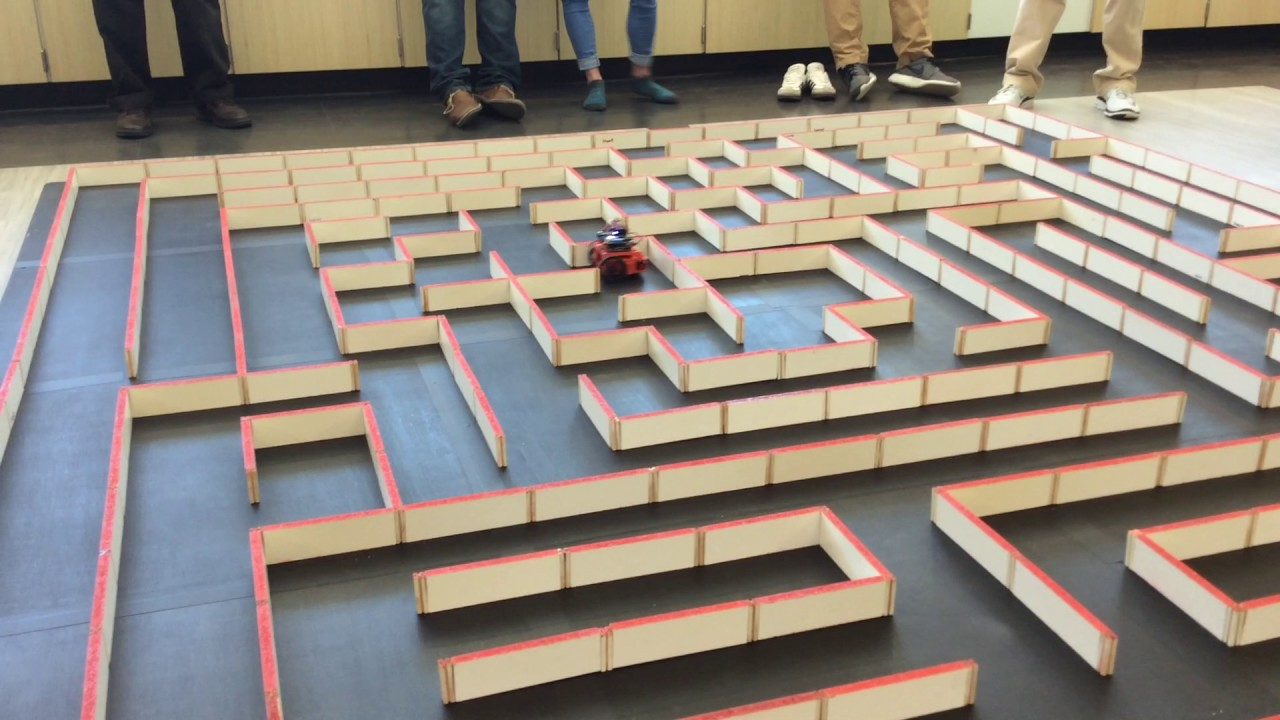
\includegraphics[height=2.5cm,keepaspectratio]{images/Maze.jpg}};}

\begin{document}

\begin{frame}
  \transfade[duration=0.1]
  \titlepage
\end{frame}

\begin{frame}{Motivation}
  \transfade[duration=0.1]
  
  \only<2>{
    \Large
    The project solves the challenge of an autonomous robot entering an unknown maze without simply following a pre-drawn line.
  }
  
  \only<3>{
    \Large
    It demonstrates the physical application of embedded algorithms, spatial mapping, and graph traversal over basic reactive control.
  }
  
  \only<4>{
    \Large
    This project leverages the group's strong software foundation in algorithms (like BFS and Flood Fill) and data structures, applying them to a complex physical constraint.
  }
  
  \only<5>{
    \Large
    The robot must map the maze, remember visited cells, calculate the shortest exit path, and return to the start.
  }
\end{frame}

\begin{frame}{Equipments \& Roles}
  \transfade[duration=0.1]
  \begin{columns}[c,onlytextwidth]
    \column{0.6\textwidth}
    
    \only<1>{
      \Large \textcolor{red}{\textbf{ATmega32 Dev Board:}}\\[0.5em]
      \normalsize
      Main low-level microcontroller for hardware interrupts and motor driving.
    }
    \only<2>{
      \Large \textcolor{red}{\textbf{ESP32 DevKit V1:}}\\[0.5em]
      \normalsize
      Coprocessor responsible for processing sensor arrays and executing pathfinding algorithms.
    }
    \only<3>{
      \Large \textcolor{red}{\textbf{L298N Motor Driver:}}\\[0.5em]
      \normalsize
      Controls the voltage and direction of the chassis motors based on microcontroller signals.
    }
    \only<4>{
      \Large \textcolor{red}{\textbf{2WD Robot Chassis Kit:}}\\[0.5em]
      \normalsize
      Provides the physical movement platform, critically requiring included wheel encoder discs.
    }
    \only<5>{
      \Large \textcolor{red}{\textbf{3x VL53L0X ToF Sensors:}}\\[0.5em]
      \normalsize
      High-precision time-of-flight sensors to detect walls on the front, left, and right sides.
    }
    \only<6>{
      \Large \textcolor{red}{\textbf{18650 Batteries \& Regulators:}}\\[0.5em]
      \normalsize
      Provides reliable portable power for the motors and distinct logic levels for the microcontrollers.
    }

    \column{0.4\textwidth}
    \raggedleft
    \only<1>{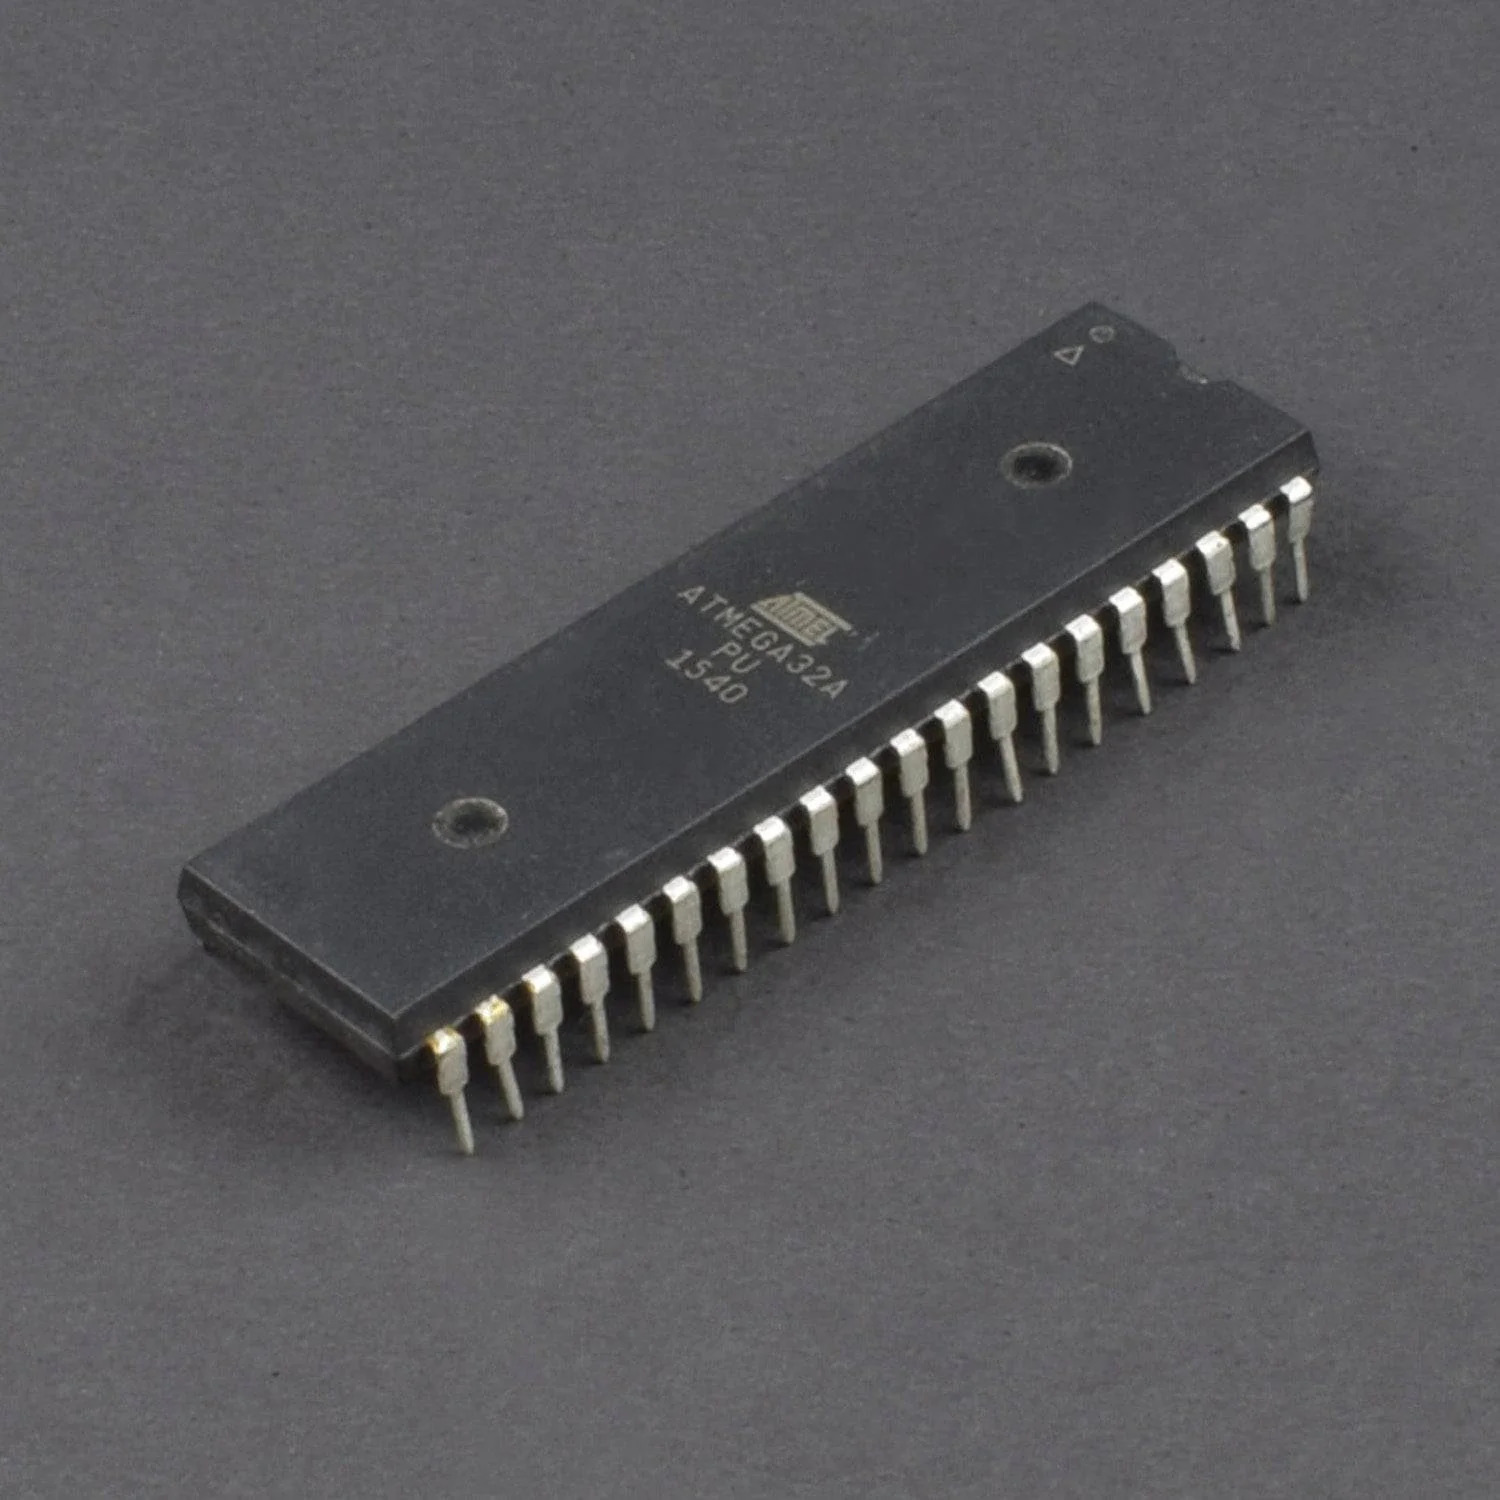
\includegraphics[width=0.95\linewidth]{images/Atmega32.jpg}}
    \only<2>{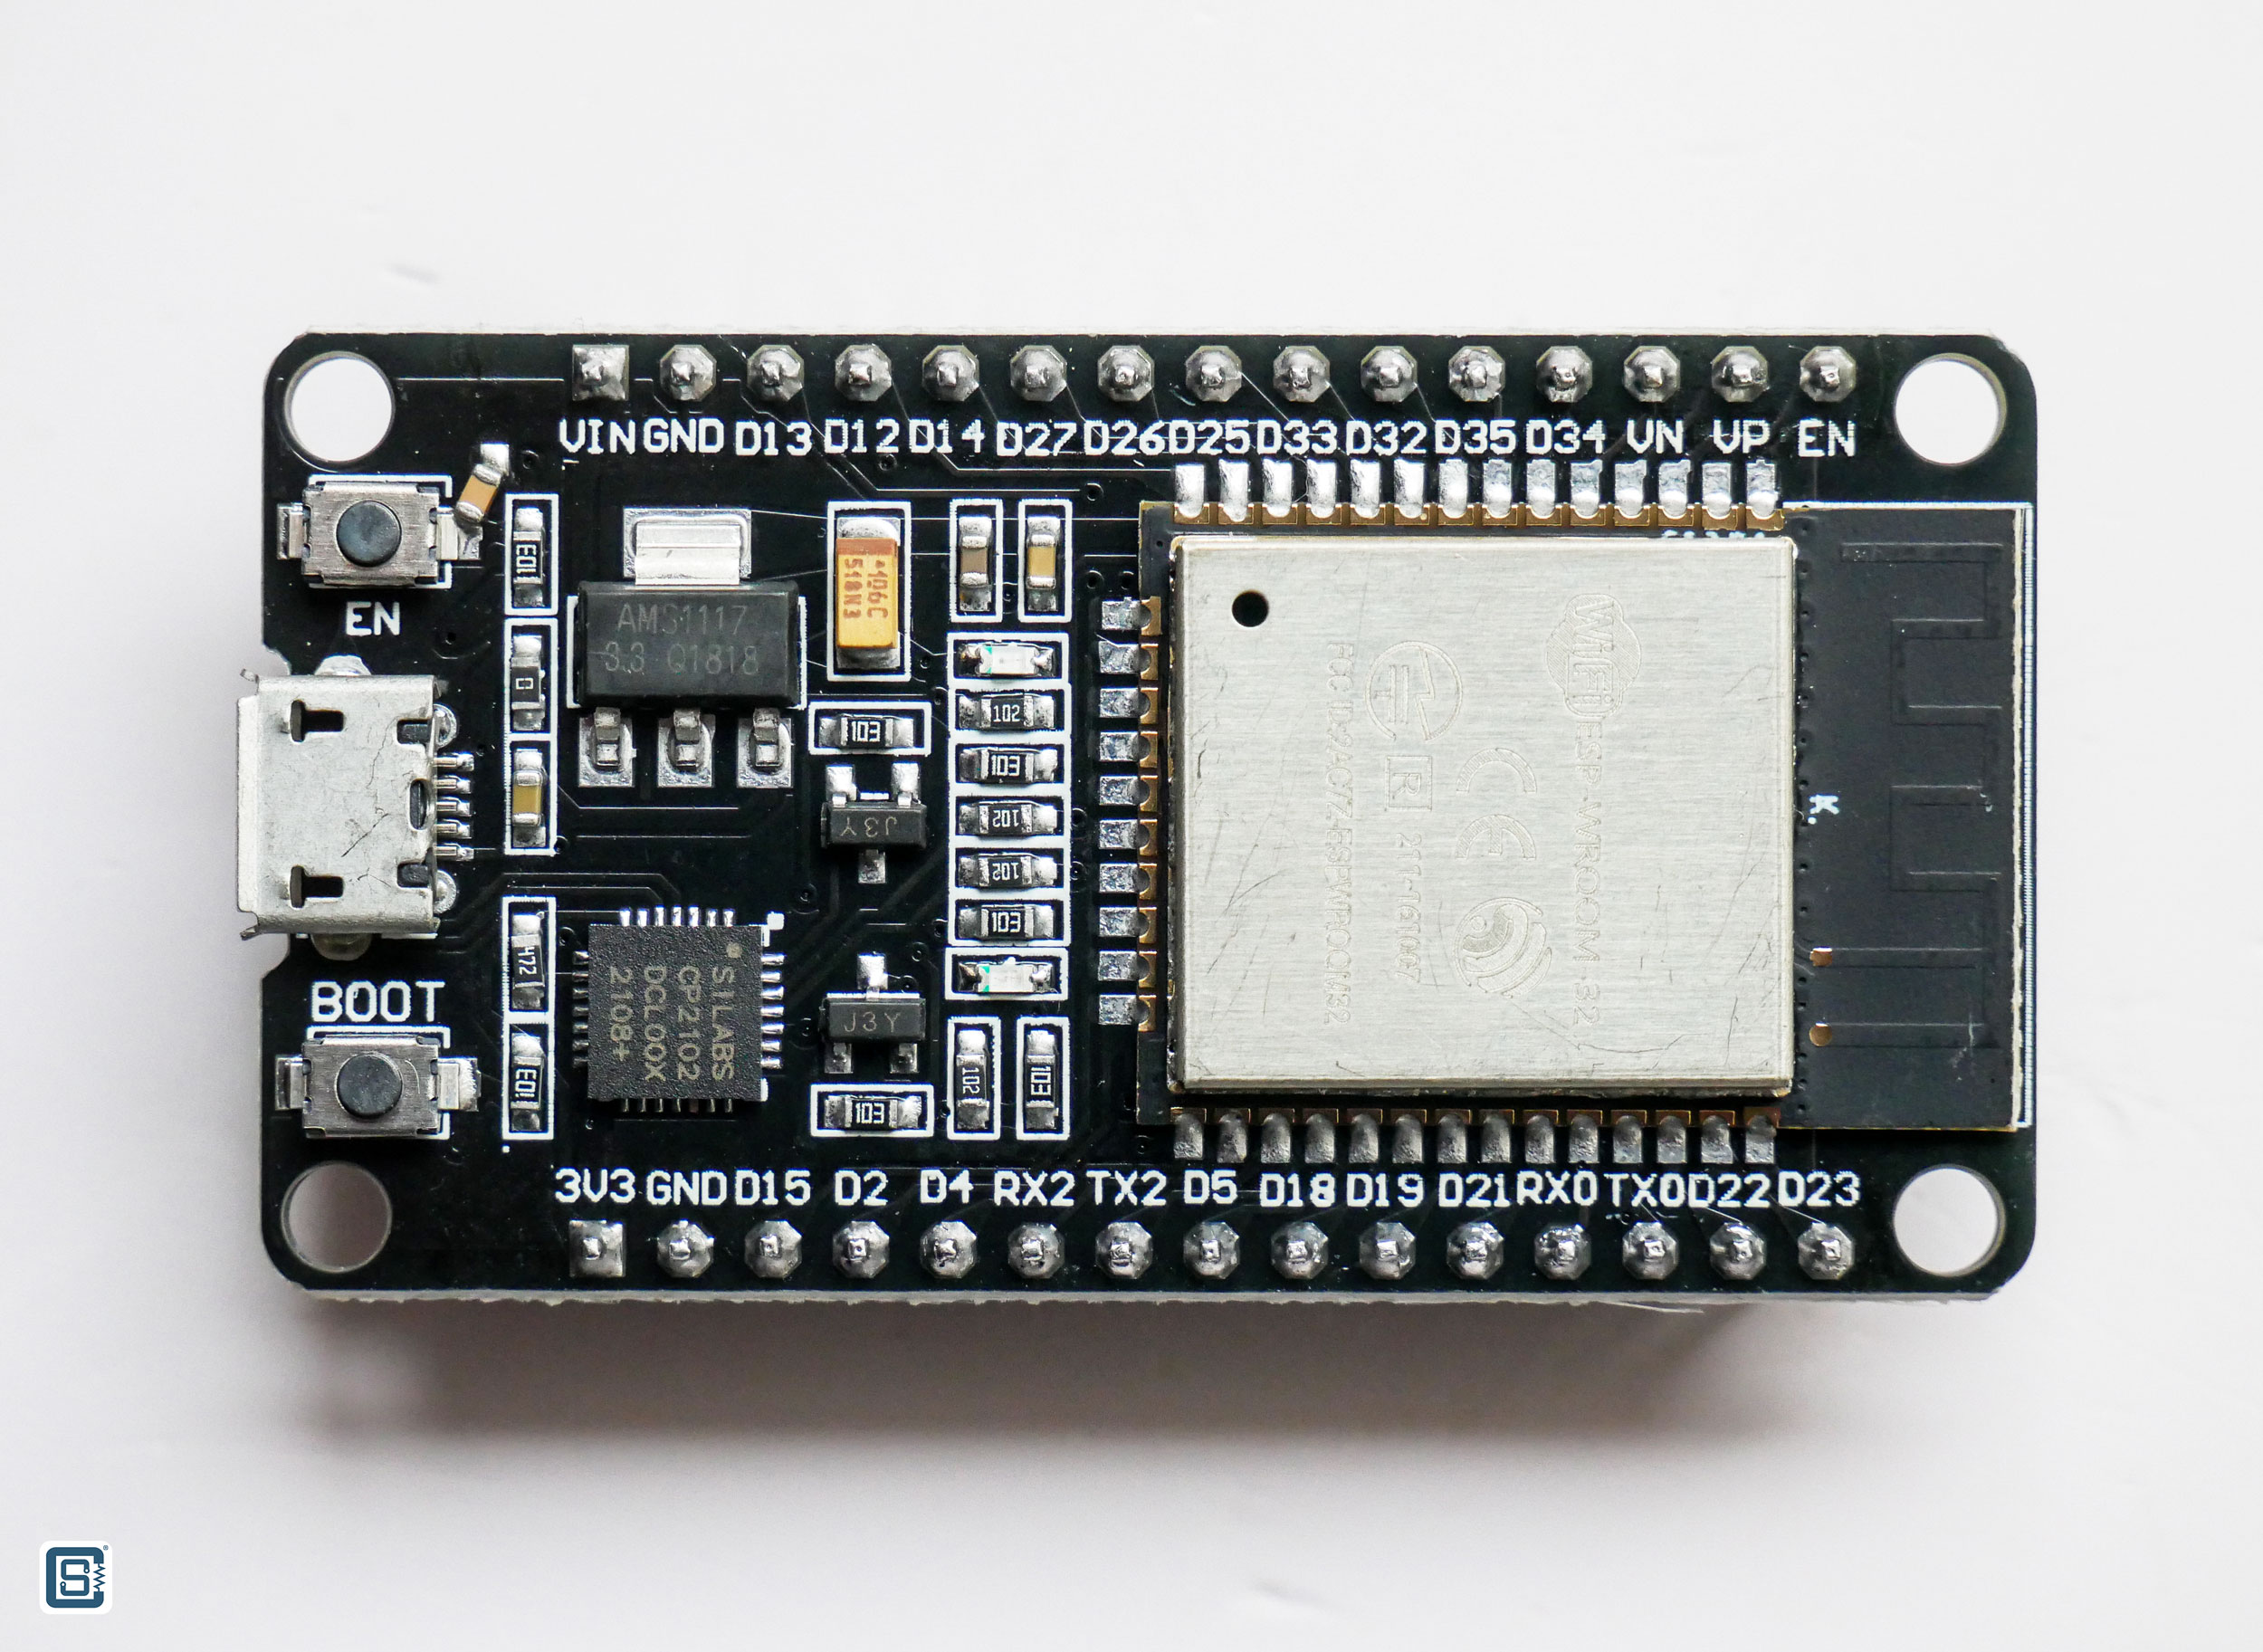
\includegraphics[width=0.95\linewidth]{images/ESP.jpg}}
    \only<3>{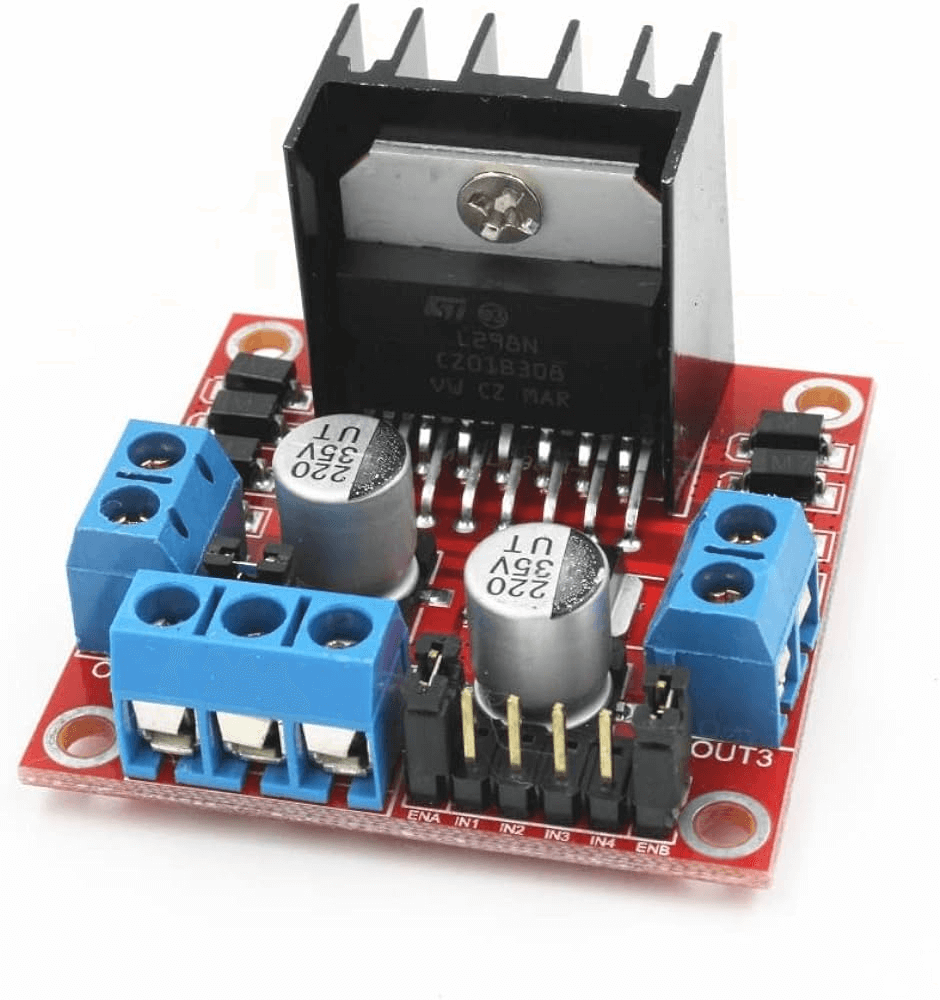
\includegraphics[width=0.95\linewidth]{images/MotorDriver.png}}
    \only<4>{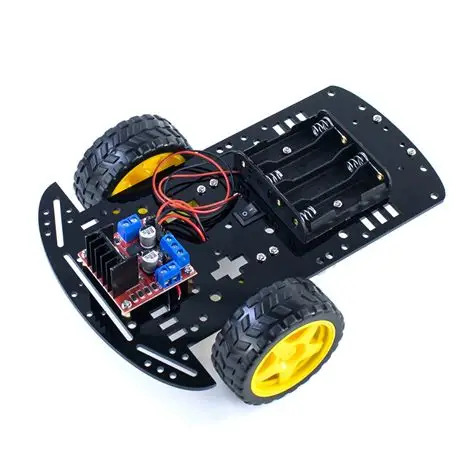
\includegraphics[width=0.95\linewidth]{images/Chassis.jpg}}
    \only<5>{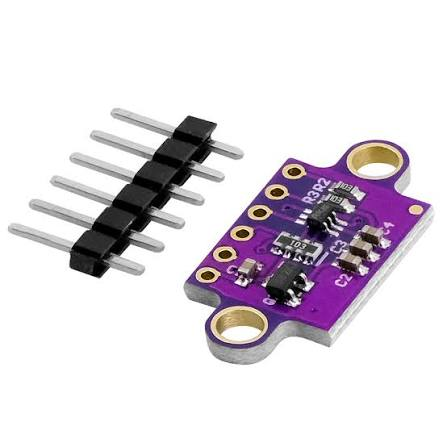
\includegraphics[width=0.95\linewidth]{images/TOFsensor.jpeg}}
    \only<6>{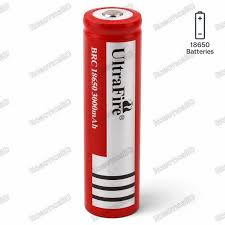
\includegraphics[width=0.95\linewidth]{images/battery.jpeg}}
  \end{columns}
\end{frame}

\begin{frame}{System Design}
  \transfade[duration=0.1]
  
  \begin{center}
    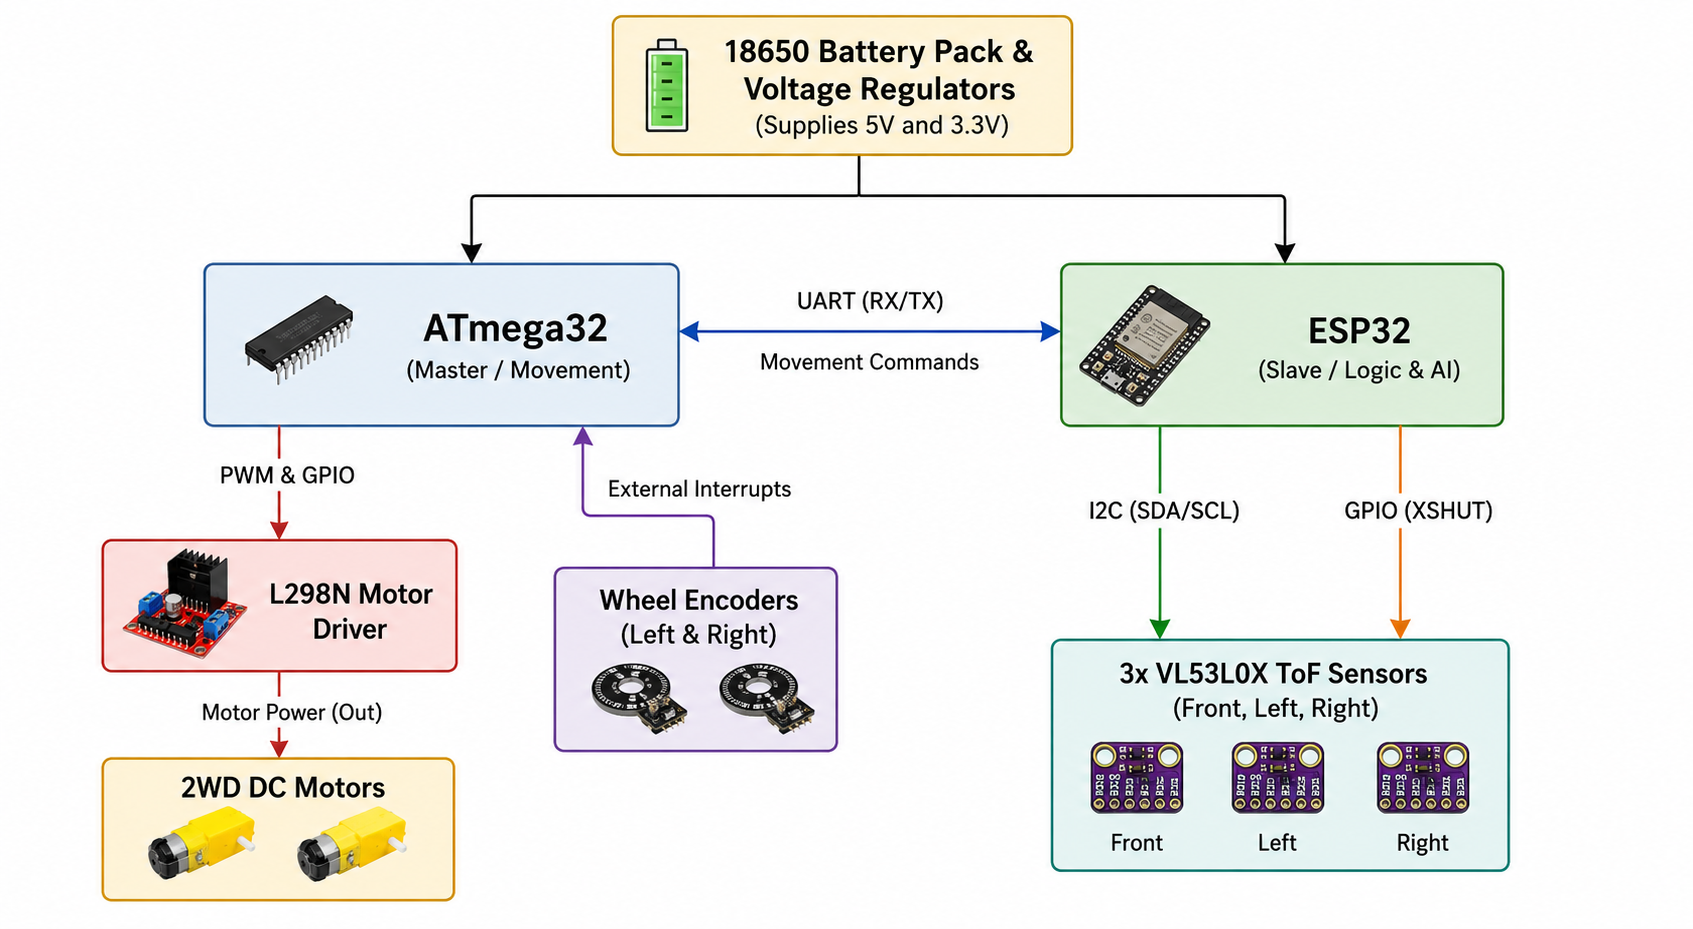
\includegraphics[height=0.55\textheight, width=\linewidth, keepaspectratio]{images/blockDiagram.png}
  \end{center}
  
  \vspace{0.5em}
  
  \only<1>{
    \small
    The system uses a master-slave configuration between the ATmega32 and the ESP32.
  }
  \only<2>{
    \small
    The ATmega32 is wired directly to the L298N motor driver and reads the wheel encoders.
  }
  \only<3>{
    \small
    The ESP32 interfaces with the three VL53L0X Time-of-Flight sensors via the I2C bus.
  }
  \only<4>{
    \small
    The ESP32 calculates movement logic and sends high-level commands (e.g., "Move Forward 1 cell") to the ATmega32 over a UART serial connection.
  }
  
  \only<5-8>{
    \textcolor{red}{\textbf{Important ATmega32 Interfaces Used:}}\\[0.5em]
    \small
    \only<5>{ \textbf{UART (RX/TX Pins):} Used to establish serial communication with the ESP32 to receive navigation commands. }
    \only<6>{ \textbf{External Interrupt Pins (INT0 / INT1):} Used to read the rapid pulse signals generated by the left and right wheel encoders to track distance. }
    \only<7>{ \textbf{PWM Channels:} Used to send variable voltage signals to the L298N driver, allowing for dynamic motor speed control via a PID algorithm. }
    \only<8>{ \textbf{Standard GPIO Pins:} Used to send basic HIGH/LOW logic to the L298N driver to control the forward and reverse direction of the motors. }
  }
\end{frame}

\begin{frame}{Role of the ATmega32}
  \transfade[duration=0.1]
  \begin{itemize}[<+->]
    \item \textcolor{red}{\textbf{Primary Tasks:}} 
      \begin{itemize}[<+->]
        \item Dedicated real-time motion controller (translates ESP32 commands to motor timings).
        \item Executes continuous PID algorithm for straight driving and exact $90^\circ$ turns.
      \end{itemize}
    \item \textcolor{red}{\textbf{Hardware Features Utilized:}}
      \begin{itemize}[<+->]
        \item \textbf{INT0/INT1:} Read encoders for real-time distance tracking.
        \item \textbf{Timers \& PWM:} Dynamic motor speed adjustments via PID.
        \item \textbf{UART \& GPIO:} Receive navigation commands and dictate motor directions.
      \end{itemize}
  \end{itemize}
\end{frame}

\begin{frame}{Use of Other Controllers (ESP32)}
  \transfade[duration=0.1]
  \begin{itemize}[<+->]
    \item \textcolor{red}{\textbf{Memory Constraint:}} The ATmega32 only has 2KB of SRAM, which severely limits its ability to store complex maze arrays while handling heavy real-time motor control.
    \item \textcolor{red} {\textbf{Tasks:}} The ESP32 handles the heavy lifting of the Flood Fill algorithm, tracks the state of the 256 cells, and manages the dynamic addressing sequence for the I2C sensors.
    \item \textcolor{red} {\textbf{Communication:}} It acts as the "brain," sending simplified directional commands to the ATmega32 over UART.
  \end{itemize}
\end{frame}

\begin{frame}{Implementation Plan: Expected Outcome}
  \transfade[duration=0.1]
  \begin{itemize}[<+->]
    \item \textcolor{red}{\textbf{Expected Outcome:}} A fully autonomous robot capable of navigating a $16 \times 16$ maze grid, mapping dead ends, and calculating the fastest route.
  \end{itemize}
\end{frame}

\begin{frame}{Implementation Plan: Project Updates}
  \transfade[duration=0.1]
  \begin{itemize}[<+->]
    \item \textcolor{red}{\textbf{Project Update 1 (Weeks 1-2):}}
    \begin{itemize}[<+->]
      \item Complete chassis assembly.
      \item Establish PC simulation of the Flood Fill algorithm.
      \item Finalize the ATmega32 PID controller so the robot can drive in a perfectly straight line for 1 meter.
    \end{itemize}
    \item \textcolor{red}{\textbf{Project Update 2 (Weeks 3-5):}}
    \begin{itemize}[<+->]
      \item Integrate the ToF sensors with the ESP32.
      \item Merge the mapping logic with the movement logic.
      \item Finalize edge-case tuning for wall-drift correction.
    \end{itemize}
  \end{itemize}
\end{frame}

\begin{frame}{Testing and Success Criteria}
  \transfade[duration=0.1]
  \textcolor{red}{\textbf{\large System Testing Methodology}}
  \vspace{0.5em}
  \begin{itemize}[<+->]
    \item \textbf{Phased Approach:} System tested in 4 phases to isolate hardware vs. algorithmic bugs.
    \item \textbf{Phase 1 (Locomotion \& PID):} Test perfectly straight 1m driving and exact $90^\circ$ turns using encoder counts.
    \item \textbf{Phase 2 (Sensor \& I2C Calibration):} Verify XSHUT addressing to prevent I2C conflicts and calibrate ToF distances.
    \item \textbf{Phase 3 (Algorithm Simulation):} Test Flood Fill algorithm on a PC simulation (virtual $16 \times 16$ grid) before flashing the ESP32.
    \item \textbf{Phase 4 (Full Integration):} Test hardware/software synchronization in scaled-down physical mazes (e.g., $4 \times 4$, $8 \times 8$).
  \end{itemize}
\end{frame}

\begin{frame}{Testing and Success Criteria}
  \transfade[duration=0.1]
  \textcolor{red}{\textbf{\large Measurable Criteria for Project Success}}
  \vspace{0.5em}
  \begin{itemize}[<+->]
    \item \textbf{Metric 1: PID Synchronization Error ($E_{PID}$)}
      \begin{itemize}[<+->]
        \item Ensures motors spin at identical rates without drifting.
        \item Formula: $E_{PID} = \left\vert{} C_{left} - C_{right} \right\vert{}$ (where $C$ = encoder pulse counts).
        \item Success: Steady-state error must approach zero during a straight-line traversal.
      \end{itemize}
    \item \textbf{Metric 2: Algorithmic Path Efficiency ($\eta_{path}$)}
      \begin{itemize}[<+->]
        \item Evaluates optimal path calculation after mapping.
        \item Formula: $\eta_{path} = \frac{S_{optimal}}{S_{traversed}}$ (Optimal cells vs. actual cells traversed).
        \item Success: Achieving $\eta_{path} = 1$, proving Flood Fill found the absolute shortest path.
      \end{itemize}
  \end{itemize}
\end{frame}

\begin{frame}{Testing and Success Criteria}
  \transfade[duration=0.1]
  \textcolor{red}{\textbf{\large Separation of Features}}
  \vspace{0.5em}
  \begin{itemize}[<+->]
    \item \textbf{Essential Features (MVP):}
      \begin{itemize}[<+->]
        \item Maintain accurate digital $(X, Y)$ coordinates and heading in memory.
        \item Autonomously map the maze and find the center in a single pass.
        \item Execute stable continuous PID motor control to navigate without crashing.
      \end{itemize}
    \item \textbf{Optional Features (Stretch Goals):}
      \begin{itemize}[<+->]
        \item \textbf{The Speed Run:} Return to the start and execute a high-speed run through the optimal path.
        \item \textbf{Live Wi-Fi Telemetry:} Broadcast the internal maze map in real-time to a laptop dashboard.
      \end{itemize}
  \end{itemize}
\end{frame}

\begin{frame}{Challenges and Future Scope}
  \transfade[duration=0.1]
  \textcolor{red}{\textbf{\large Technical and Hardware-Related Challenges}}
  \vspace{0.5em}
  \begin{itemize}[<+->]
    \item \textbf{Wheel Slip \& Trajectory Drift:} 
      \begin{itemize}[<+->]
        \item Physical motors never spin at perfectly identical speeds.
        \item Solution: Highly tuned PID control using wheel encoders to constantly correct drift.
      \end{itemize}
    \item \textbf{I2C Address Conflicts:} 
      \begin{itemize}[<+->]
        \item All three VL53L0X sensors share the same default I2C address.
        \item Solution: Sequentially wake sensors via XSHUT pins and dynamically assign unique addresses.
      \end{itemize}
    \item \textbf{ATmega32 Memory Limits (2KB SRAM):} 
      \begin{itemize}[<+->]
        \item High risk of exhausting memory when storing maze states and processing interrupts.
        \item Solution: Use efficient bitwise operations and offload Flood Fill logic to the ESP32.
      \end{itemize}
  \end{itemize}
\end{frame}

\begin{frame}{Challenges and Future Scope}
  \transfade[duration=0.1]
  \textcolor{red}{\textbf{\large Future Scope and Improvements}}
  \vspace{0.5em}
  \begin{itemize}[<+->]
    \item \textbf{Live Wi-Fi Telemetry (Dashboard):}
      \begin{itemize}[<+->]
        \item Broadcast the ESP32's internal maze map over Wi-Fi.
        \item Visualize robot coordinates and walls in real-time on a React/Node.js frontend.
      \end{itemize}
    \item \textbf{The Optimal Speed Run:}
      \begin{itemize}[<+->]
        \item Expand the software to a complete multi-pass solver.
        \item After mapping, return to start and execute a high-speed run through the calculated shortest route.
      \end{itemize}
    \item \textbf{Sensor Fusion (IMU Integration):}
      \begin{itemize}[<+->]
        \item Integrate an MPU6050 (Accelerometer \& Gyroscope).
        \item Fuse gyro data with wheel encoders for flawless straight headings and exactly $90^\circ$ turns.
      \end{itemize}
  \end{itemize}
\end{frame}

\end{document}
